\title{Heuristic Analysis for Isolation Game}
\date{\today}

\documentclass[10pt]{article}
\usepackage{graphicx}
\begin{document}
\maketitle

A minimax algorithm with alpha-beta pruning was implemented on three isolation agents. Each agent was designed to assign scores to different board states (nodes) using a different heuristic. The three custom heuristics were designed as follows:

\begin{enumerate}
\item \textbf{Custom\_Agent\_1:} This heuristic allows the agent to make tactical decisions based on the occupancy of the corner and wall squares. It rewards moving into wall and corner squares at the beginning of the game, and then places a penalty on using these squares as the game progresses (they are easily trapped later in the game). At the same time, there is a reward available throughout the game for occupying non-wall and non-corner squares as these (potentially) allow flexible movement in more directions. A score is calculated for both the agent and the opponent using this metric and the idea is to maximise the difference between the agent and the opponent with a $70 : 30$ weighting for $\textrm{corners} : \textrm{walls}$.
\item \textbf{Custom\_Agent\_2:} This heuristic will try to force a board partition early on by awarding a high score to those boxes close to the main vertical and horizontal.
\item \textbf{Custom\_Agent\_3:} This heuristic is an adjustment to the improved\_score heuristic from the lectures whereby the agent's reward is weighted by an aggression factor that is close to 0 at the start of the game and close to 1 at the end of the game. This means the agent is rewarded for keeping their moves open at the start (avoiding early isolation) and then in the endgame they are rewarded for aggressively trying to isolate their opponent.
\end{enumerate}

The three custom agents then competed against each other and an improved alpha-beta pruning agent, \textbf{AB\_Improved}, in a tournament competition against seven different agents using a variety of scoring heuristics involving random play, minimax and minimax with alpha-beta pruning. Each match consisted of ten different games and the number of wins and losses against each opposition agent is recorded in the table and graph below:

\begin{figure}
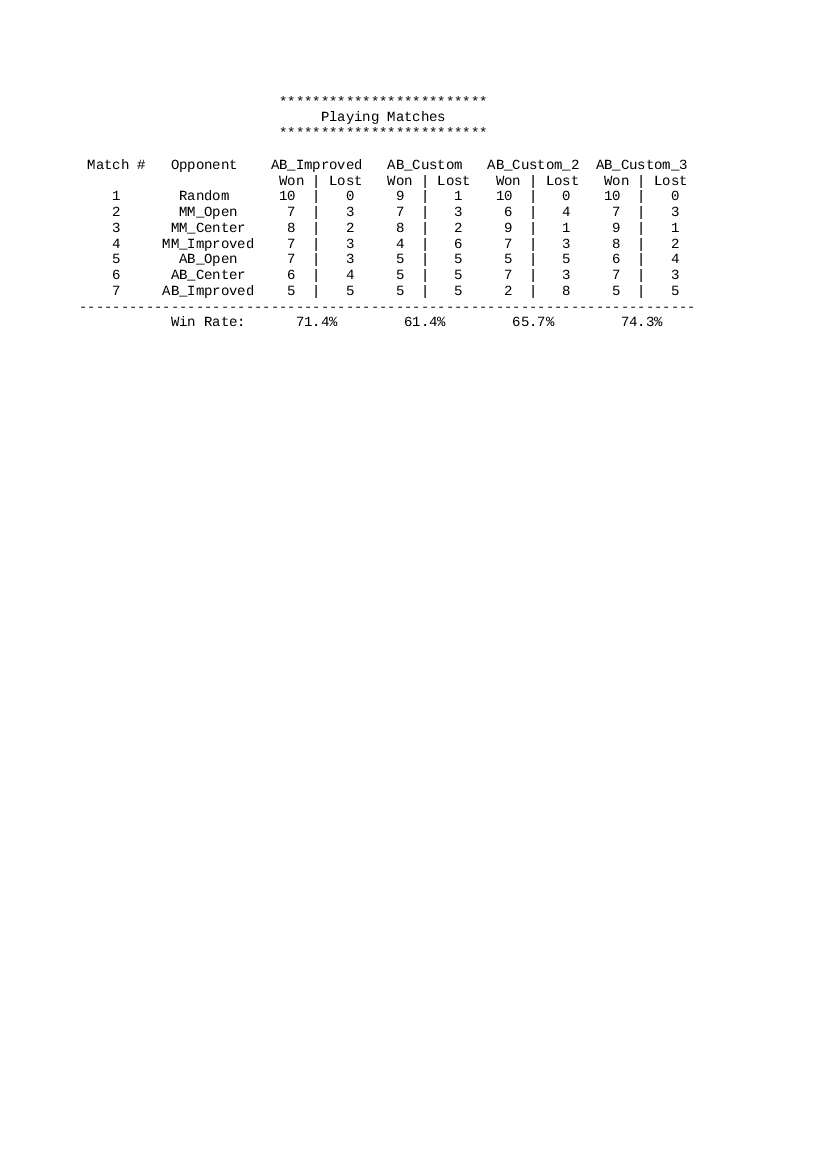
\includegraphics[scale=1,, trim = {4cm, 20cm, 0, 2cm}, clip]{output.png}
\end{figure}
           
\begin{figure}
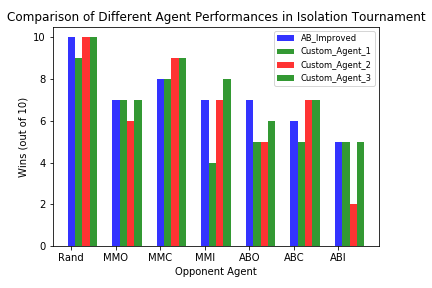
\includegraphics[scale=1]{agents.png}
\end{figure}

\newpage

We can see from the table that all three agents achieve a win rate above 60\%. However, it appears that \textbf{Custom\_Agent\_3} is the best. This agent uses the following scoring metric:
\begin{equation}
\textrm{reward} = \textrm{own\_moves} - \frac{25 - \textrm{total\_moves}}{25} \times \textrm{opp\_moves}
\end{equation}
The reasons for this agent's success are threefold:
\begin{enumerate}
\item  From my experience playing Isolation, it is important to avoid being cornered early on. \textbf{Custom\_Agent\_3} does this by placing a high importance on keeping own\_moves high at the start of the game.
\item From my experience playing Isolation, it is important to play aggressively at the end as the number of available moves rapidly decreases in the endgame. \textbf{Custom\_Agent\_3} does this by placing a high importance on limiting opp\_moves at the end of the game.
\item It has the highest win rate of the three custom agents. It beats the other agents in every single match except for the match against \textbf{AB\_Open} in which case \textbf{AB\_Improved} does marginally better. However, on the whole, \textbf{Custom\_Agent\_3} is consistently beating the other agents.
\end{enumerate}
For the above reasons, \textbf{Custom\_Agent\_3} is the one that should be used for future gameplay
\end{document}